\chapter{Introducción específica} % Main chapter title
\label{Chapter2}

A continuación, se explican los frameworks, arquitecturas y bibliotecas utilizadas en el trabajo, los conjuntos de datos utilizados para el entrenamiento y validación de los modelos, y por último, una breve mención a la infraestructura de cómputo utilizada. 

\section{Frameworks y bibliotecas}

Las Redes Neuronales Profundas (DNN, del inglés \textit{Deep Neural Networks}) son el modelo fundamental de Aprendizaje Profundo. El objetivo de una DNN es aproximar una función $f^*$, definiendo un mapeo $\mathbf{y}=f(\mathbf{x};\mathbf{\theta})$ del cual se aprenden los parámetros $\mathbf{\theta}$ para lograr la mejor aproximación de la función objetivo. La unidad básica de las DNN es el perceptrón, el cual aplica una transformación lineal seguido de una transformación no-lineal, llamada activación. Decimos redes neuronales, debido a que se aplican múltiples perceptrones en capas consecutivas. Podemos pensar a las DNN como "máquinas de aproximación de funciones, diseñadas para obtener generalización estadísitica" \citep{GOODFELLOW_DEEPLEARNING}. Esto las hace interesantes para su aplicación en la resolución del primer problema planteado en este trabajo: la estimación rápida de PLC, aprovechando la basta cantidad de datos acumulados.

También es de interés en este trabajo analizar la aplicación de reducción de dimensionalidad a partir de algunos \textit{set} de \textit{features}. Para realizar esto, se utiliza una arquitectura \textit{encoder-decoder}. Esta arquitectura se encuentra representada en la figura \ref{fig:embedding}, donde se observa una primera DNN, llamada \textit{encoder}, que reduce de dimensión el \textit{input} al vector \textit{feature} o \textit{embedding}, y luego una segunda DNN, llamada \textit{decoder}, que reconstruye a partir del \textit{embedding} el \textit{input}. Esto permite representar la misma información con una menor dimensionalidad, capturando las características representativas del vector de entrada.

Por otro lado, para el planteo de una nueva metodología de estimación de CHF utilizando ML, nos centramos en dos arquitecturas particulares derivadas de las DNN. En el trabajo de Raissi, Perdikaris y Karniadakis \citep{RAISSI2019} se presentan las PINN, las cuales permiten obtener una función de pérdida que busque cumplir una ecuación diferencial en derivadas parciales (PDE, del inglés \textit{Partial Differential Equation}), además de la función de pérdida respecto de los datos tabulados para entrenamiento. 

En la figura \ref{fig:pinn} se presenta un esquema general de una arquitectura PINN. Se tiene una DNN que predice $\hat{u}$ a partir de las entradas $\mathbf{x}$ y $t$. Luego se computa por medio de diferenciación automática las derivadas necesarias de $\hat{u}$, como pueden ser la derivada temporal, el gradiente, el laplaciano, etc. Luego, se calcula el error cuadrático medio (MSE, del inglés \textit{Mean Squared Error}) del residuo del ajuste de los datos rotulados, el residuo de la ecuación de gobierno, el residuo de las condiciones de borde y el residuo de las condiciones iniciales, para luego computar la pérdida global y su gradiente para aplicar el algorítmo de aprendizaje basado en gradiente.

Este enfoque se puede denominar como \textit{grey box}, ya que el modelo, si bien tiene una componente desconocida al entrenarse y ajustar sus parámetros, tiene a la función de pérdida de forma conocida que nos da información de su funcionamiento interno. Los modelos de DNN típicamente se llaman \textit{black box}, mientras que modelos más tradicionales de resolución de problemas físicos como las diferencias finitas, los elementos finitos o los volúmenes finitos, son considerados modelos \textit{white box}. Esta característica es interesante para su aplicación en el ámbito nuclear, ya que este requiere de alta certeza en las predicciones debido a los altos estándares de seguridad que se deben cumplir.

Por otro lado, en el trabajo de Meng y Karniadakis \citep{MENG2020} se presenta una arquitectura novedosa de redes neuronales, llamadas Redes Neuronales Profundas de Multi-Fidelidad (MFDNN, del inglés \textit{Multi-Fidelity Deep Neural Networks}). Esta arquitectura permite considerar conjuntos de datos de distinta fidelidad, por ejemplo, datos obtenidos a partir de ensayos experimentales (alta fidelida, disponibilidad acotada o baja), datos obtenidos a partir de ensayos numéricos (baja fidelidad, disponibilidad acotada o alta), datos de ensayos experimentales en geometrías o condiciones diferentes (baja fidelidad, disponibilidad alta), etc. Para realizar esto, propone la hipótesis de que los datos de alta fidelidad tienen una relación no-lineal con los datos de baja fidelidad de la forma: 
\begin{equation}
	y_H = \mathcal{F}(\mathbf{x}, y_L),
\end{equation}
siendo $y_H$ la información de alta fidelidad, $y_L$ la información de baja fidelidad y $\mathbf{x}$ los datos de entrada. Esta relación no-lineal es posible de representar con una DNN, por lo que se construye una arquitectura que consiste de una DNN que estima $y_L$ a partir de $\mathbf{x}$, y luego otra que estima $y_H$ a partir de $\hat{y_L}$ y $\mathbf{x}$. En la figura \ref{fig:mfdnn} se esquematiza esta arquitectura. Debe notarse que el trabajo original propone estimar la relación entre alta y baja fidelidad por medio de dos redes, una lineal ($\mathcal{F}_l$) y otra no-lineal ($\mathcal{F}_{nl}$), pero esto es redundante, ya que una red no-lineal puede capturar la relación lineal.

Si agregamos una función de pérdida basada en lo propuesto en las PINN, obtenemos la variante informada por física de las MFDNN, las Redes Neuronales Informadas por Física de Multi-Fidelidad (MFPINN, del inglés \textit{Multi-Fidelity Physics-Informed Neural Networks}). Esto es lo que se representa en la figura \ref{fig:mfdnn} con el cómputo de las derivadas de $\hat{y_H}$ y el posterior cálculo de $f_e$.

Para realizar el desarrollo de las arquitecturas mencionadas, en este trabajo se utiliza la librería PyTorch \citep{PYTORCH} \citep{PYTORCH_WEBSITE}.

% \pagebreak
% \begin{equation}
% 	\text{MSE} = \text{MSE}_{y_L} + \text{MSE}_{y_H} + \text{MSE}_{f_e} + \lambda \sum \beta_i^2
% \end{equation}

\begin{figure}[htbp]
	\centering
	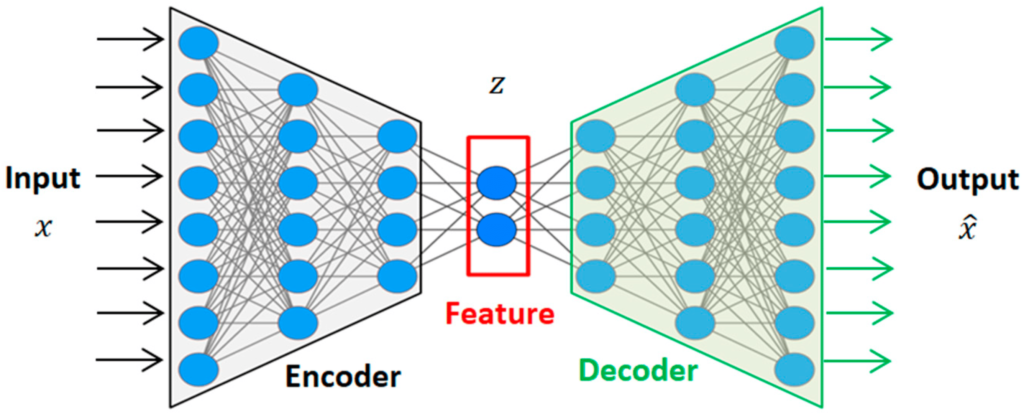
\includegraphics[width=.7\textwidth]{./Figures/encoder-decoder.png}
	\caption{Esquema de arquitectura encoder-decoder\protect\footnotemark{}.}
	\label{fig:embedding}
\end{figure}
\footnotetext{Imagen tomada de \href{https://muditb.com/neural-encoders-from-autoencoders-to-modern-retrieval-architectures/}{https://muditb.com}.}

\begin{figure}[htbp]
	\centering
	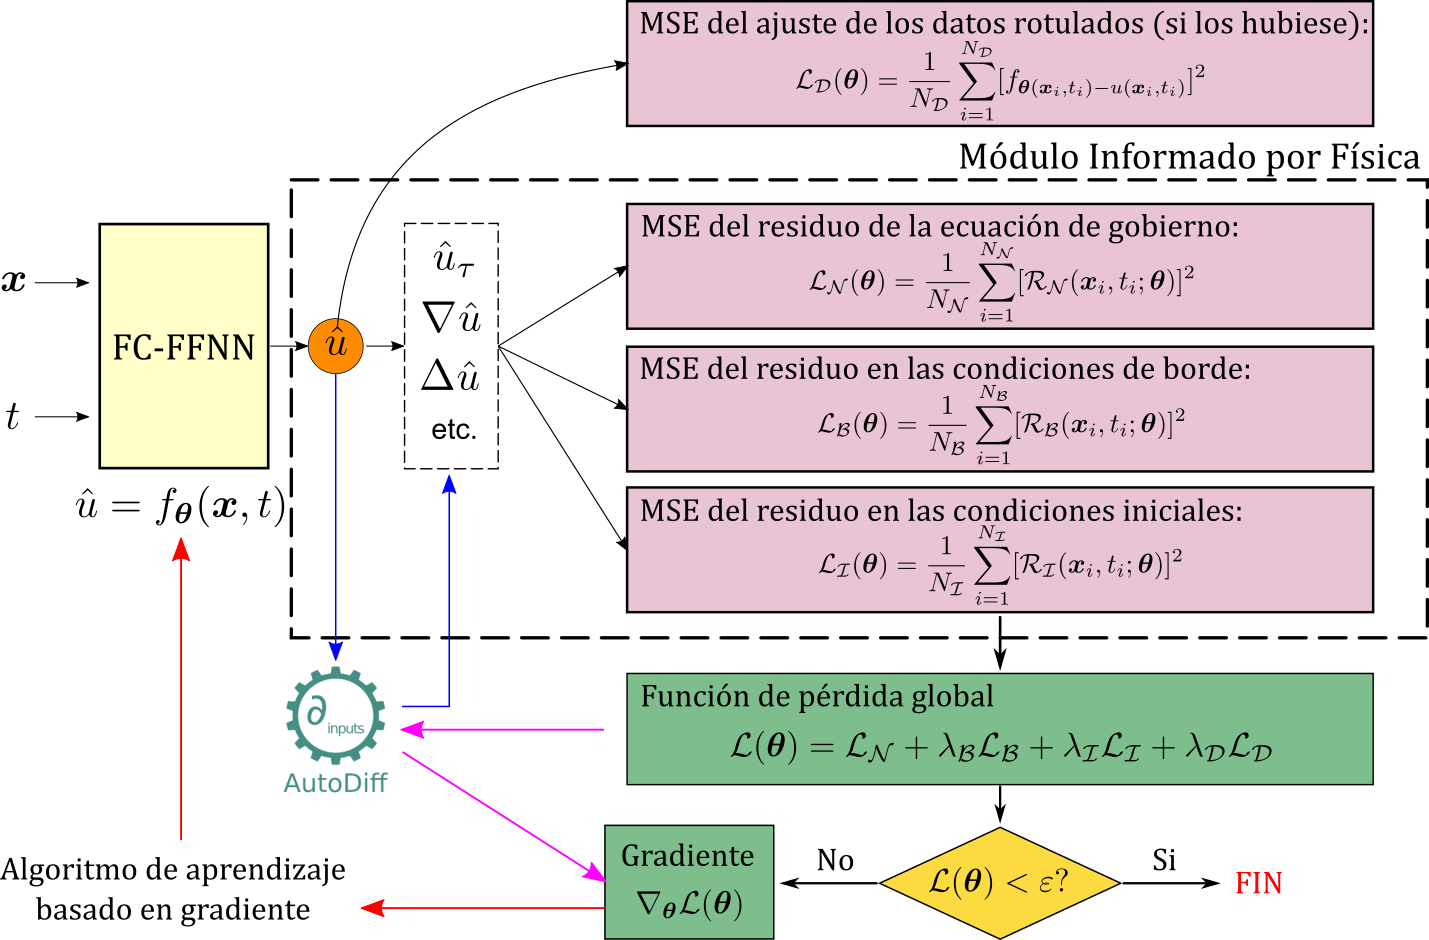
\includegraphics[width=.9\textwidth]{./Figures/pinn.png}
	\caption{Esquema de PINN\protect\footnotemark{}.}
	\label{fig:pinn}
\end{figure}
\footnotetext{Imagen tomada del curso \textit{Redes Neuronales Informadas por Física} de la CEIA.}

\begin{figure}[htbp]
	\centering
	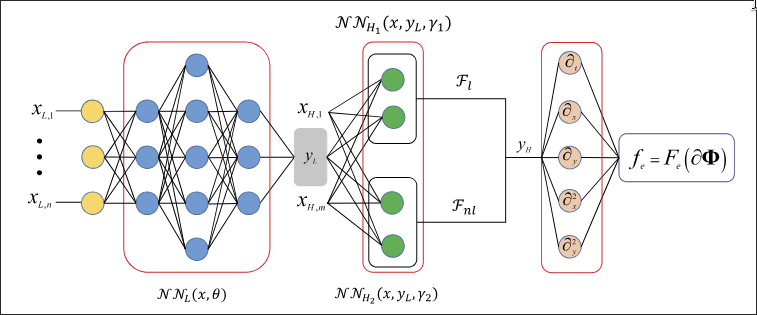
\includegraphics[width=.9\textwidth]{./Figures/mfdnn.png}
	\caption{Esquema de MFDNN y MFPINN\protect\footnotemark{}.}
	\label{fig:mfdnn}
\end{figure}
\footnotetext{Imagen tomada de Meng y Karniadakis \citep{MENG2020}.}

\pagebreak

\section{Datasets y datos de entrenamiento}

En cuanto a los datos de entrenamiento, debemos dividir esta sección en los datos utilizados para la estimación de las PLC y para la estimación de CHF.

Para la estimación de PLC, se utilizan datos de simulaciones realizadas por la División de Diseño Termohidráulico de la Gerencia de Análisis de Seguridad y Diseño del Núcleo (GASyDN) de Nucleoeléctrica Argentina S.A. (NA-SA), los cuales son de carácter confidencial. Los datos fueron generados con el código de simulación termohidráulica de subcanales COBRA3-CP \citep{cobra3cp}, a partir de estados del reactor calculados en las simulaciones de estrategias de recambio de combustibles. De las salidas de las simulaciones de COBRA3-CP se extrae:
\begin{itemize}
	\item Perfil axial de potencia.
	\item Perfil de potencia por barra combustible.
	\item Mínimo DNBR.
	\item Temperatura de entrada.
	\item Presión de salida.
	\item Potencia total.
	\item Zona hidráulica.
\end{itemize}

Por otro lado, para la estimación de CHF, se tiene múltiples fuentes de datos. Se incluyen: los datos de ensayos en un tubo usados por Groeneveld en su LUT 2006 \citep{GROENEVELD2007}, obtenidos de \citep{USNRC2019NUREGKM0011}; los datos de ensayos sobre el \textit{bundle} de la CNA-UII realizados por la Universidad de Columbia \citep{recopilacion_columbia}; y el replicado de los ensayos de Columbia con COBRA3-CP, ampliando la cantidad de puntos de ensayo. Estas últimas dos fuentes de datos son de carácter confidencial. 

Los datos de ensayos en un tubo tienen los siguientes datos disponibles: diámetro, longitud, presión a la salida, flujo másico, título termodinámico a la salida, entalpía a la entrada, flujo de calor y temperatura de entrada. 

Los datos de los ensayos de Columbia tienen los siguientes datos disponibles: presión a la salida, temperatura de entrada, flujo másico, flujo de calor, título termodinámico a la salida y diferencia de presión a la entrada.

\section{Infraestructura de cómputo}

En cuanto a infraestructura de cómputo, debido al carácter confidencial de los datos utilizados, se opta por realizar todo el proceso de entrenamiento en un entorno local. Para ello se dispone de dos computadoras, una provista por la empresa NA-SA, con una placa gráfica NVIDIA A2000 y 32GB de RAM, y otra de uso personal del autor, con una placa gráfica NVIDIA RTX 3090 y 64GB de RAM. Ambas computadoras tienen capacidad apta para el trabajo en cuestión. 